\documentclass[14pt]{extbook}
\usepackage{multicol, enumerate, enumitem, hyperref, color, soul, setspace, parskip, fancyhdr} %General Packages
\usepackage{amssymb, amsthm, amsmath, latexsym, units, mathtools} %Math Packages
\everymath{\displaystyle} %All math in Display Style
% Packages with additional options
\usepackage[headsep=0.5cm,headheight=12pt, left=1 in,right= 1 in,top= 1 in,bottom= 1 in]{geometry}
\usepackage[usenames,dvipsnames]{xcolor}
\usepackage{dashrule}  % Package to use the command below to create lines between items
\newcommand{\litem}[1]{\item#1\hspace*{-1cm}\rule{\textwidth}{0.4pt}}
\pagestyle{fancy}
\lhead{Makeup Progress Quiz 3}
\chead{}
\rhead{Version A}
\lfoot{1648-1753}
\cfoot{}
\rfoot{Summer C 2021}
\begin{document}

\begin{enumerate}
\litem{
Solve the quadratic equation below. Then, choose the intervals that the solutions $x_1$ and $x_2$ belong to, with $x_1 \leq x_2$.\[ 20x^{2} -81 x + 81 = 0 \]\begin{enumerate}[label=\Alph*.]
\item \( x_1 \in [1.7, 1.9] \text{ and } x_2 \in [2, 3.75] \)
\item \( x_1 \in [0.69, 0.84] \text{ and } x_2 \in [4.7, 6.1] \)
\item \( x_1 \in [0.47, 0.65] \text{ and } x_2 \in [5.74, 7.32] \)
\item \( x_1 \in [35.93, 36.06] \text{ and } x_2 \in [44.58, 45.52] \)
\item \( x_1 \in [0.37, 0.51] \text{ and } x_2 \in [8.3, 10.3] \)

\end{enumerate} }
\litem{
Factor the quadratic below. Then, choose the intervals that contain the constants in the form $(ax+b)(cx+d); b \leq d.$\[ 36x^{2} -47 x + 15 \]\begin{enumerate}[label=\Alph*.]
\item \( a \in [26.9, 28.3], \hspace*{5mm} b \in [-7, -2], \hspace*{5mm} c \in [-1.1, 3.4], \text{ and } \hspace*{5mm} d \in [-8, 4] \)
\item \( a \in [8.3, 9.1], \hspace*{5mm} b \in [-7, -2], \hspace*{5mm} c \in [1.5, 4.9], \text{ and } \hspace*{5mm} d \in [-8, 4] \)
\item \( a \in [2.5, 7.2], \hspace*{5mm} b \in [-7, -2], \hspace*{5mm} c \in [6.4, 8.6], \text{ and } \hspace*{5mm} d \in [-8, 4] \)
\item \( a \in [-1.6, 1.4], \hspace*{5mm} b \in [-33, -24], \hspace*{5mm} c \in [-1.1, 3.4], \text{ and } \hspace*{5mm} d \in [-20, -19] \)
\item \( \text{None of the above.} \)

\end{enumerate} }
\litem{
Graph the equation below.\[ f(x) = -(x+4)^2 - 12 \]\begin{enumerate}[label=\Alph*.]
\begin{multicols}{2}\item 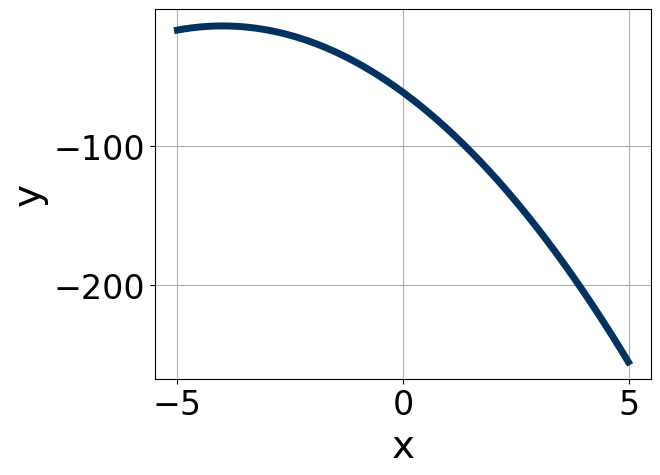
\includegraphics[width = 0.3\textwidth]{../Figures/quadraticEquationToGraphAA.png}\item 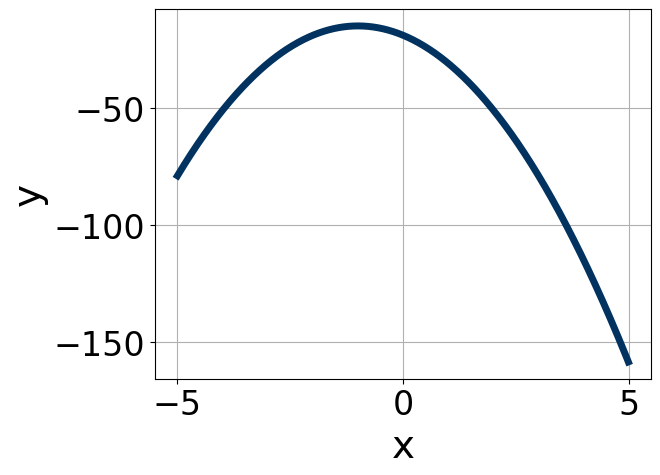
\includegraphics[width = 0.3\textwidth]{../Figures/quadraticEquationToGraphBA.png}\item 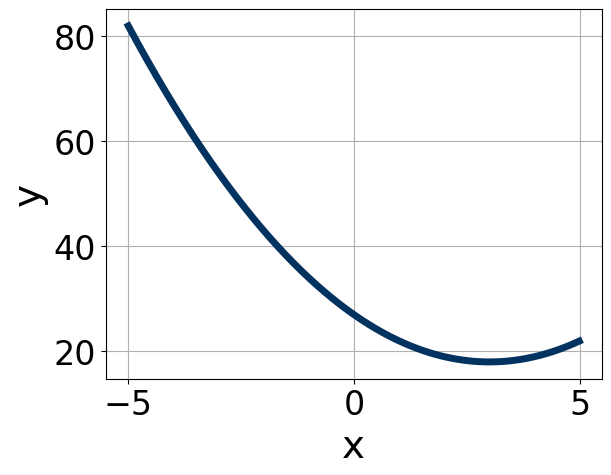
\includegraphics[width = 0.3\textwidth]{../Figures/quadraticEquationToGraphCA.png}\item 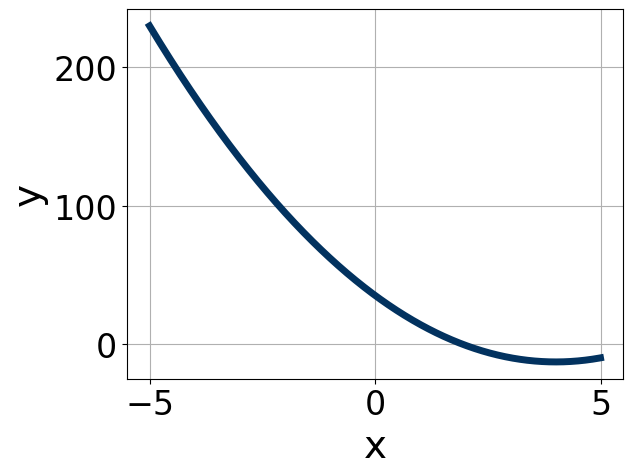
\includegraphics[width = 0.3\textwidth]{../Figures/quadraticEquationToGraphDA.png}\end{multicols}\item None of the above.
\end{enumerate} }
\litem{
Factor the quadratic below. Then, choose the intervals that contain the constants in the form $(ax+b)(cx+d); b \leq d.$\[ 36x^{2} +60 x + 25 \]\begin{enumerate}[label=\Alph*.]
\item \( a \in [4.6, 7.7], \hspace*{5mm} b \in [3, 7], \hspace*{5mm} c \in [5.5, 6.3], \text{ and } \hspace*{5mm} d \in [5, 12] \)
\item \( a \in [2, 5.9], \hspace*{5mm} b \in [3, 7], \hspace*{5mm} c \in [10.2, 14.5], \text{ and } \hspace*{5mm} d \in [5, 12] \)
\item \( a \in [0.1, 1.2], \hspace*{5mm} b \in [21, 33], \hspace*{5mm} c \in [-1.6, 1.6], \text{ and } \hspace*{5mm} d \in [26, 40] \)
\item \( a \in [10.1, 13.4], \hspace*{5mm} b \in [3, 7], \hspace*{5mm} c \in [2.7, 3.7], \text{ and } \hspace*{5mm} d \in [5, 12] \)
\item \( \text{None of the above.} \)

\end{enumerate} }
\litem{
Write the equation of the graph presented below in the form $f(x)=ax^2+bx+c$, assuming  $a=1$ or $a=-1$. Then, choose the intervals that $a, b,$ and $c$ belong to.
\begin{center}
    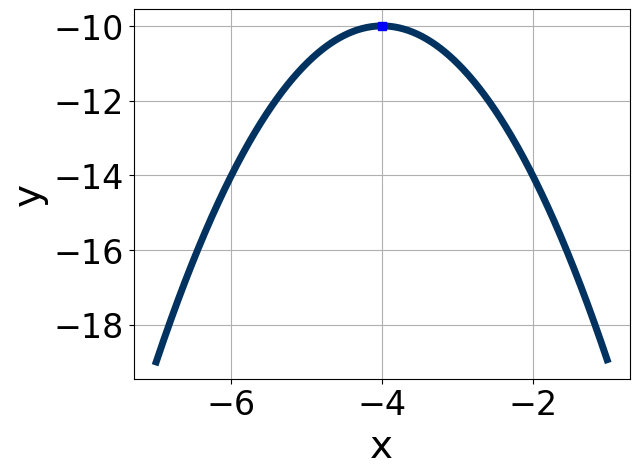
\includegraphics[width=0.5\textwidth]{../Figures/quadraticGraphToEquationCopyA.png}
\end{center}
\begin{enumerate}[label=\Alph*.]
\item \( a \in [1, 7], \hspace*{5mm} b \in [-9, -5], \text{ and } \hspace*{5mm} c \in [11, 15] \)
\item \( a \in [1, 7], \hspace*{5mm} b \in [7, 9], \text{ and } \hspace*{5mm} c \in [15, 20] \)
\item \( a \in [-3, 0], \hspace*{5mm} b \in [7, 9], \text{ and } \hspace*{5mm} c \in [-19, -17] \)
\item \( a \in [-3, 0], \hspace*{5mm} b \in [-9, -5], \text{ and } \hspace*{5mm} c \in [-19, -17] \)
\item \( a \in [1, 7], \hspace*{5mm} b \in [7, 9], \text{ and } \hspace*{5mm} c \in [11, 15] \)

\end{enumerate} }
\litem{
Solve the quadratic equation below. Then, choose the intervals that the solutions belong to, with $x_1 \leq x_2$ (if they exist).\[ -19x^{2} +8 x + 2 = 0 \]\begin{enumerate}[label=\Alph*.]
\item \( x_1 \in [-11.46, -11.16] \text{ and } x_2 \in [3.2, 3.42] \)
\item \( x_1 \in [-0.45, -0.08] \text{ and } x_2 \in [0.35, 0.79] \)
\item \( x_1 \in [-14.57, -14.06] \text{ and } x_2 \in [14.54, 15.14] \)
\item \( x_1 \in [-0.88, -0.54] \text{ and } x_2 \in [-0.02, 0.31] \)
\item \( \text{There are no Real solutions.} \)

\end{enumerate} }
\litem{
Solve the quadratic equation below. Then, choose the intervals that the solutions belong to, with $x_1 \leq x_2$ (if they exist).\[ 13x^{2} -10 x -2 = 0 \]\begin{enumerate}[label=\Alph*.]
\item \( x_1 \in [-2.52, -1.09] \text{ and } x_2 \in [11.78, 12.16] \)
\item \( x_1 \in [-1.11, -0.77] \text{ and } x_2 \in [-0.53, 0.3] \)
\item \( x_1 \in [-14.1, -13.45] \text{ and } x_2 \in [14.46, 15.58] \)
\item \( x_1 \in [-0.62, 0.01] \text{ and } x_2 \in [0.92, 1.01] \)
\item \( \text{There are no Real solutions.} \)

\end{enumerate} }
\litem{
Solve the quadratic equation below. Then, choose the intervals that the solutions $x_1$ and $x_2$ belong to, with $x_1 \leq x_2$.\[ 10x^{2} -57 x + 54 = 0 \]\begin{enumerate}[label=\Alph*.]
\item \( x_1 \in [11.46, 12.14] \text{ and } x_2 \in [44.94, 46.17] \)
\item \( x_1 \in [0.76, 1.06] \text{ and } x_2 \in [5.46, 6.34] \)
\item \( x_1 \in [1.48, 1.53] \text{ and } x_2 \in [1.82, 4.42] \)
\item \( x_1 \in [0.99, 1.31] \text{ and } x_2 \in [4.31, 4.7] \)
\item \( x_1 \in [0.13, 0.65] \text{ and } x_2 \in [8.76, 9.75] \)

\end{enumerate} }
\litem{
Write the equation of the graph presented below in the form $f(x)=ax^2+bx+c$, assuming  $a=1$ or $a=-1$. Then, choose the intervals that $a, b,$ and $c$ belong to.
\begin{center}
    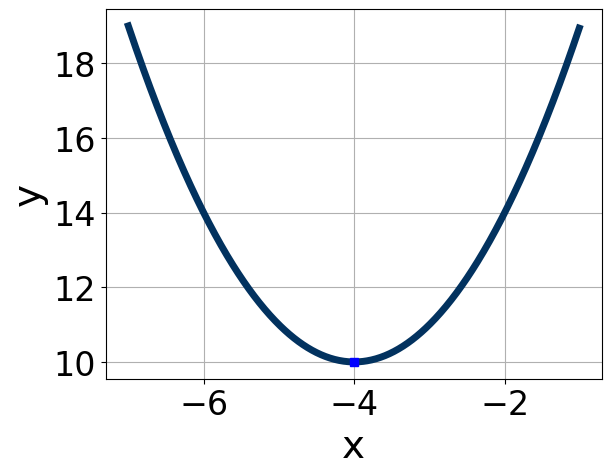
\includegraphics[width=0.5\textwidth]{../Figures/quadraticGraphToEquationA.png}
\end{center}
\begin{enumerate}[label=\Alph*.]
\item \( a \in [-0.6, 1.3], \hspace*{5mm} b \in [-6, -3], \text{ and } \hspace*{5mm} c \in [11, 13] \)
\item \( a \in [-1.1, 0.2], \hspace*{5mm} b \in [-6, -3], \text{ and } \hspace*{5mm} c \in [3, 6] \)
\item \( a \in [-0.6, 1.3], \hspace*{5mm} b \in [-6, -3], \text{ and } \hspace*{5mm} c \in [-4, -1] \)
\item \( a \in [-1.1, 0.2], \hspace*{5mm} b \in [1, 6], \text{ and } \hspace*{5mm} c \in [3, 6] \)
\item \( a \in [-0.6, 1.3], \hspace*{5mm} b \in [1, 6], \text{ and } \hspace*{5mm} c \in [11, 13] \)

\end{enumerate} }
\litem{
Graph the equation below.\[ f(x) = -(x-2)^2 - 19 \]\begin{enumerate}[label=\Alph*.]
\begin{multicols}{2}\item 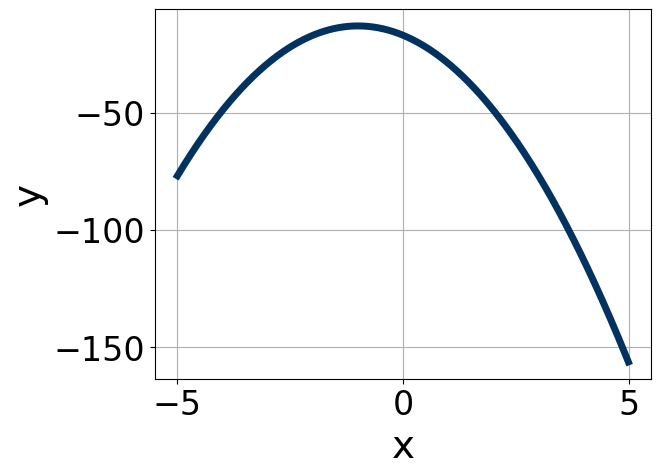
\includegraphics[width = 0.3\textwidth]{../Figures/quadraticEquationToGraphCopyAA.png}\item 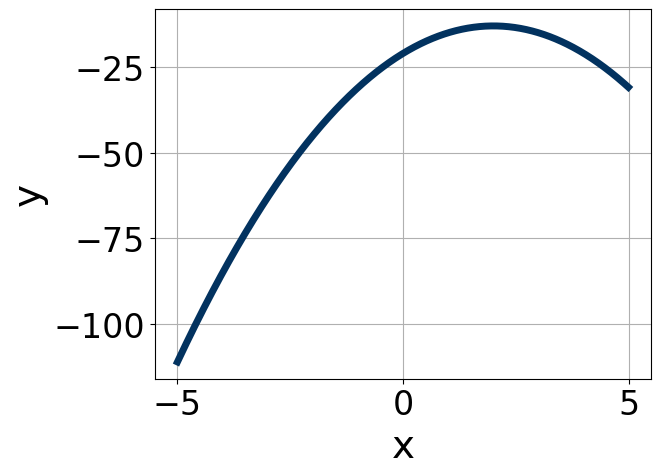
\includegraphics[width = 0.3\textwidth]{../Figures/quadraticEquationToGraphCopyBA.png}\item 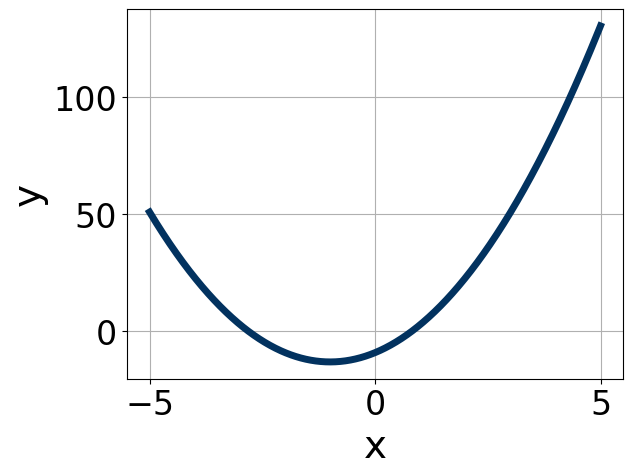
\includegraphics[width = 0.3\textwidth]{../Figures/quadraticEquationToGraphCopyCA.png}\item 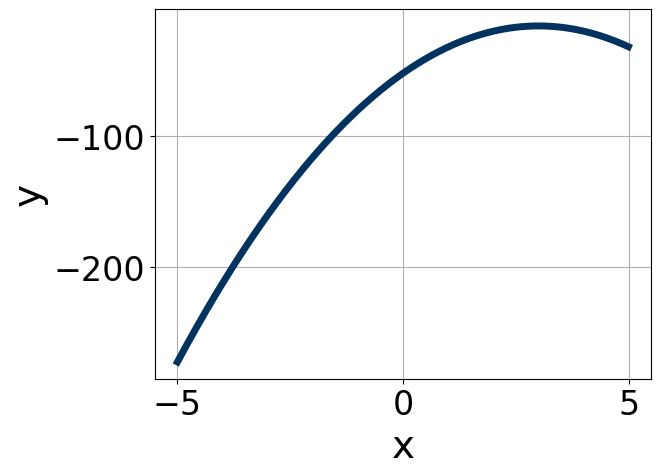
\includegraphics[width = 0.3\textwidth]{../Figures/quadraticEquationToGraphCopyDA.png}\end{multicols}\item None of the above.
\end{enumerate} }
\end{enumerate}

\end{document}